\section{Algorithms}
%%%%%%%%%%%%%%%%%%%%%%%%%%%%%%%%%%%%%%%%%%%%%%%%%%%%%%%%%%%%%%%%%%%%%%%%%%%%%

\subsection{Hierarchical Optimistic Optimization Algorithm}
% introduction and summary
% description of covering tree
% summarized pseudo code of the HOO algorithm
% discussion of regret bounds
% implementation notes.

The Hierarchical Optimistic Optimization (HOO) algorithm is a
no-regret algorithm for the case when the ``arms'' form a generic
measurable space $\cX$, and when each arm $x \in \cX$ is associated
with a fixed distribution $f(x)$ of rewards with finite support. Much
like the UCB algorithm, the HOO algorithm seeks to accurately estimate
the reward function where it has high value, while loosely estimating
the reward function where it has low value. This is accomplished by
incrementally building a covering of the space $\cX$ with fine
subdivisions where rewards are high, and coarse subdivisions
elsewhere. These coverings are maintained in a tree data structure
called a \emph{covering tree}. In the covering tree, the root covers
all of $\cX$; other nodes represent finer subsets of $\cX$. A
deterministic rule based on values stored at each node of the tree is
used to descend the tree until a leaf is reached. This leaf represents
a subset of $\cX$ from which to (arbitrarily) select the next arm. The
reward for that arm is used to update the values associated with all
nodes along the path from chosen leaf to root. The regret bounds of
the algorithm are in terms of a local smoothness property at the
maxima of the mean-reward function $f$.

\subsubsection{Covering Tree}\label{sss:coverTree}
The HOO algorithm requires an infinite binary tree where each node
represents a subset of $\cX$. We denote the $i^{th}$ node at level
$h$ as $(h,i)$, and its two children as $(h+1, 2i-1)$ and $(h+1,
2i)$. The subset of $\cX$ associated with node $(h,i)$ is denoted
as $\cP_{(h,i)}$.

The covering tree is required to satisfy two properties:
\begin{align*}
  \cP_{(1,0} &= \cX\\
  \cP_({h,i}) &= \cP_({h+1,2i-1}) \cup \cP_({h+1,2i})
\end{align*}

TODO: Can talk about diameters, and size of coverings here.

\subsubsection{HOO Algorithm}
The HOO algorithm operates by maintaining a collection of subsets
which cover the space $\cX$, along with an upper bound of the expected
reward of points in each subset that holds in high probability. These
subsets are maintained in the covering tree. Each time an arm is
selected, a new and finer subset is added to the covering tree. Arms
are selected by optimistically ``zeroing in'' on regions of high
expected reward. In this way, the tree develops fine granularity
around subsets of $\cX$ with high expected reward, and coarse
granularity around subsets of $\cX$ with low expected reward.

%% The HOO algorithm works in two parts. First, to select an arm, a
%% downward pass is made through the covering tree until a leaf is
%% reached. An arm $x \in \cP_{leaf}$ is selected, and a reward is
%% received.. In the second part of the algorithm, an upward pass from
%% leaf to root is made. The values of all nodes along this path are u

\begin{algorithm}
  \SetKwData{Left}{left}\SetKwData{This}{this}\SetKwData{Up}{up}
  \SetKwFunction{Union}{Union}\SetKwFunction{FindCompress}{FindCompress}
  \SetKwInOut{Input}{input}\SetKwInOut{Output}{output}
  %initialization
  %$ \cT \leftarrow \{ (0,1) \}$\;
  %$B_{1,2} \leftarrow \infty$ \;
  %$B_{2,2} \leftarrow \infty$ \;
  \For{$i=1,2,\dots$}{
    leaf $\leftarrow$ descendToLeaf(root)\;
    %currentNode $\leftarrow$ root\;
    %% \While{currentNode has been instantiated}{
    %%   $B_{left} \leftarrow$ Bvalue(leftChild(currentNode))\;
    %%   $B_{right} \leftarrow$ Bvalue(rightChild(currentNode))\;
    %%   \uIf{$B_{left} > B_{right}$}{
    %%     currentNode $\leftarrow$ leftChild(currentNode)\;
    %%   }
    %%   \Else{
    %%     currentNode $\leftarrow$ rightChild(currentNode)\;
    %%   }
    %% }
    %instantiate currentNode\;
    %Choose arm $x$ in $\cP_{currentNode}$ and play it\;
    arm $\leftarrow$ chooseArm(leaf)\;
    $Y \leftarrow$ getReward(arm)\;
    %Choose arm $x$ in $\cP_{leaf}$ and play it\;
    %Receive reward $Y$\;
    %$\cT \leftarrow \cT \cup$ currentNode \;
    updateValues(leaf)\;
    %Update values on path from leaf to root\;
    %% \ForAll{$(h,i) \in$ pathToRoot(currentNode)}{
    %%   $T_{h,i} \leftarrow T_{h,i} + 1$\;
    %%   $\hat{\mu}_{h,i} \leftarrow (1 - \frac{1}{T_{h,i}})
    %%   \hat{\mu}_{h,i} + \frac{Y}{T_{h,i}}$\;
    %% }
    %% \ForAll{$(h,i) \in$ pathToRoot(currentNode)}{
    %%   $U_{h,i} \leftarrow \hat{\mu}_{h,i} + \sqrt{(2 \ln n) / T_{h,i}}
    %%   + \nu_1 \rho^{h}$\;
    %% }
    %$B_{H+1, 2I-1} \leftarrow \infty$\;
    %$B_{H+1, 2I} \leftarrow -\infty$\;
    %$\cT' \leftarrow \cT$\;
    %% \While{$\cT' \neq \{ (0,1) \}$}{
    %%   $(h,i) \leftarrow$ {\sc leaf}$(\cT')$\;
    %%   $B_{h,i} \leftarrow \min \{ U_{h,i}, \max B_{h+1,
    %%         2i-1},B_{h+1, 2i}  \}$ \;
    %%   $\cT' \leftarrow \cT' \setminus \{ (h,i) \} $ \;
    %% }
  }
  \caption{Hierarchical Optimistic Optimization}\label{alg:hooShort}
\end{algorithm}

Full pseudo-code is given in \algref{alg:hoo}.

``Node selection works by comparing $B$-values and always choosing the
node with the highest $B$-value.''

\begin{align*}
  \hat{\mu}_{h,i} &= \text{avg. reward received by } v_{h,i} \text{
    and its descendants.}\\
\end{align*}

\subsubsection{Regret Bounds}
The mean-payoff function $f$ is assumed to satisfy the condition that
$\forall \; x,y \in \cX$,
\begin{equation*}
  f^* - f(y) \leq f^* - f(x) + \max \{f^* - f(x), l(x,y) \}
\end{equation*}
for some dissimilarity function $l(\cdot, \cdot)$. Such a function is
called \emph{weakly Lipschitz}. Note that this amounts to requiring
(one-sided) Lipschitzness at the maxima, while only requiring a looser
condition at other points. The further a point is from the maxima, the
looser is the requirement on smoothness.



\subsubsection{Implementation}
The primary component of the implementation is the cover tree. When
$\cX$ is an n-dimensional rectangle in $\reals^n$, the covering tree
can be implemented as a binary tree in which each node represents a
rectangular region, and where the two children of each node are
defined by splitting their parent's region along some coordinate axis
(e.g., splitting the longest side). Incidentally, this is known as a
$kD$-tree data structure. While this is sufficient for such spaces as
the unit hypercube, it is also sufficient for several other spaces
which can be defined by points in a unit hypercube, such as an
n-dimensional sphere (in polar coordinates) or torus.

%%%%%%%%%%%%%%%%%%%%%%%%%%%%%%%%%%%%%%%%%%%%%%%%%%%%%%%%%%%%%%%%%%%%%
\subsection{Zooming Algorithm}
When the number of arms is infinite, additional assumptions are needed
about the relationship between the arms. For instance, arms that are
\emph{close} should produce similar results. The Zooming Algorithm is
defined to work in any example where the arms form a metric space. In
each phase, certain arms are chosen to be \emph{active}, and the
algorithm chooses which arm to play from these active arms.

The Zooming Algorithm is composed of multiple phases, each of which is
composed of $2^{i_{ph}}$ rounds, where $i_{ph}$ is the current phase
number. In a given round, you \emph{activate} an arm if that arm is
not covered by another arm. Each arm covers a radius defined by
$r_t(v):=\sqrt{8*i_{ph}/(2+n_t(v)))}$ where $v$ is the active arm, and
$n_t(v)$ is the number of times a given arm has been chosen at time
$t$. Each time an arm is played, its radius shrinks, and at the
beginning of each round, you \emph{activate} arms until you have a
complete covering using a \emph{covering oracle}. This oracle can
either return an uncovered arm, or state that there is no such
arm. After the space is covered, you play the arm with the optimal
index, defined as $I_t(v):=\mu_t(v)+2*r_t(v)$

\begin{figure}[!ht]
  \begin{center}
    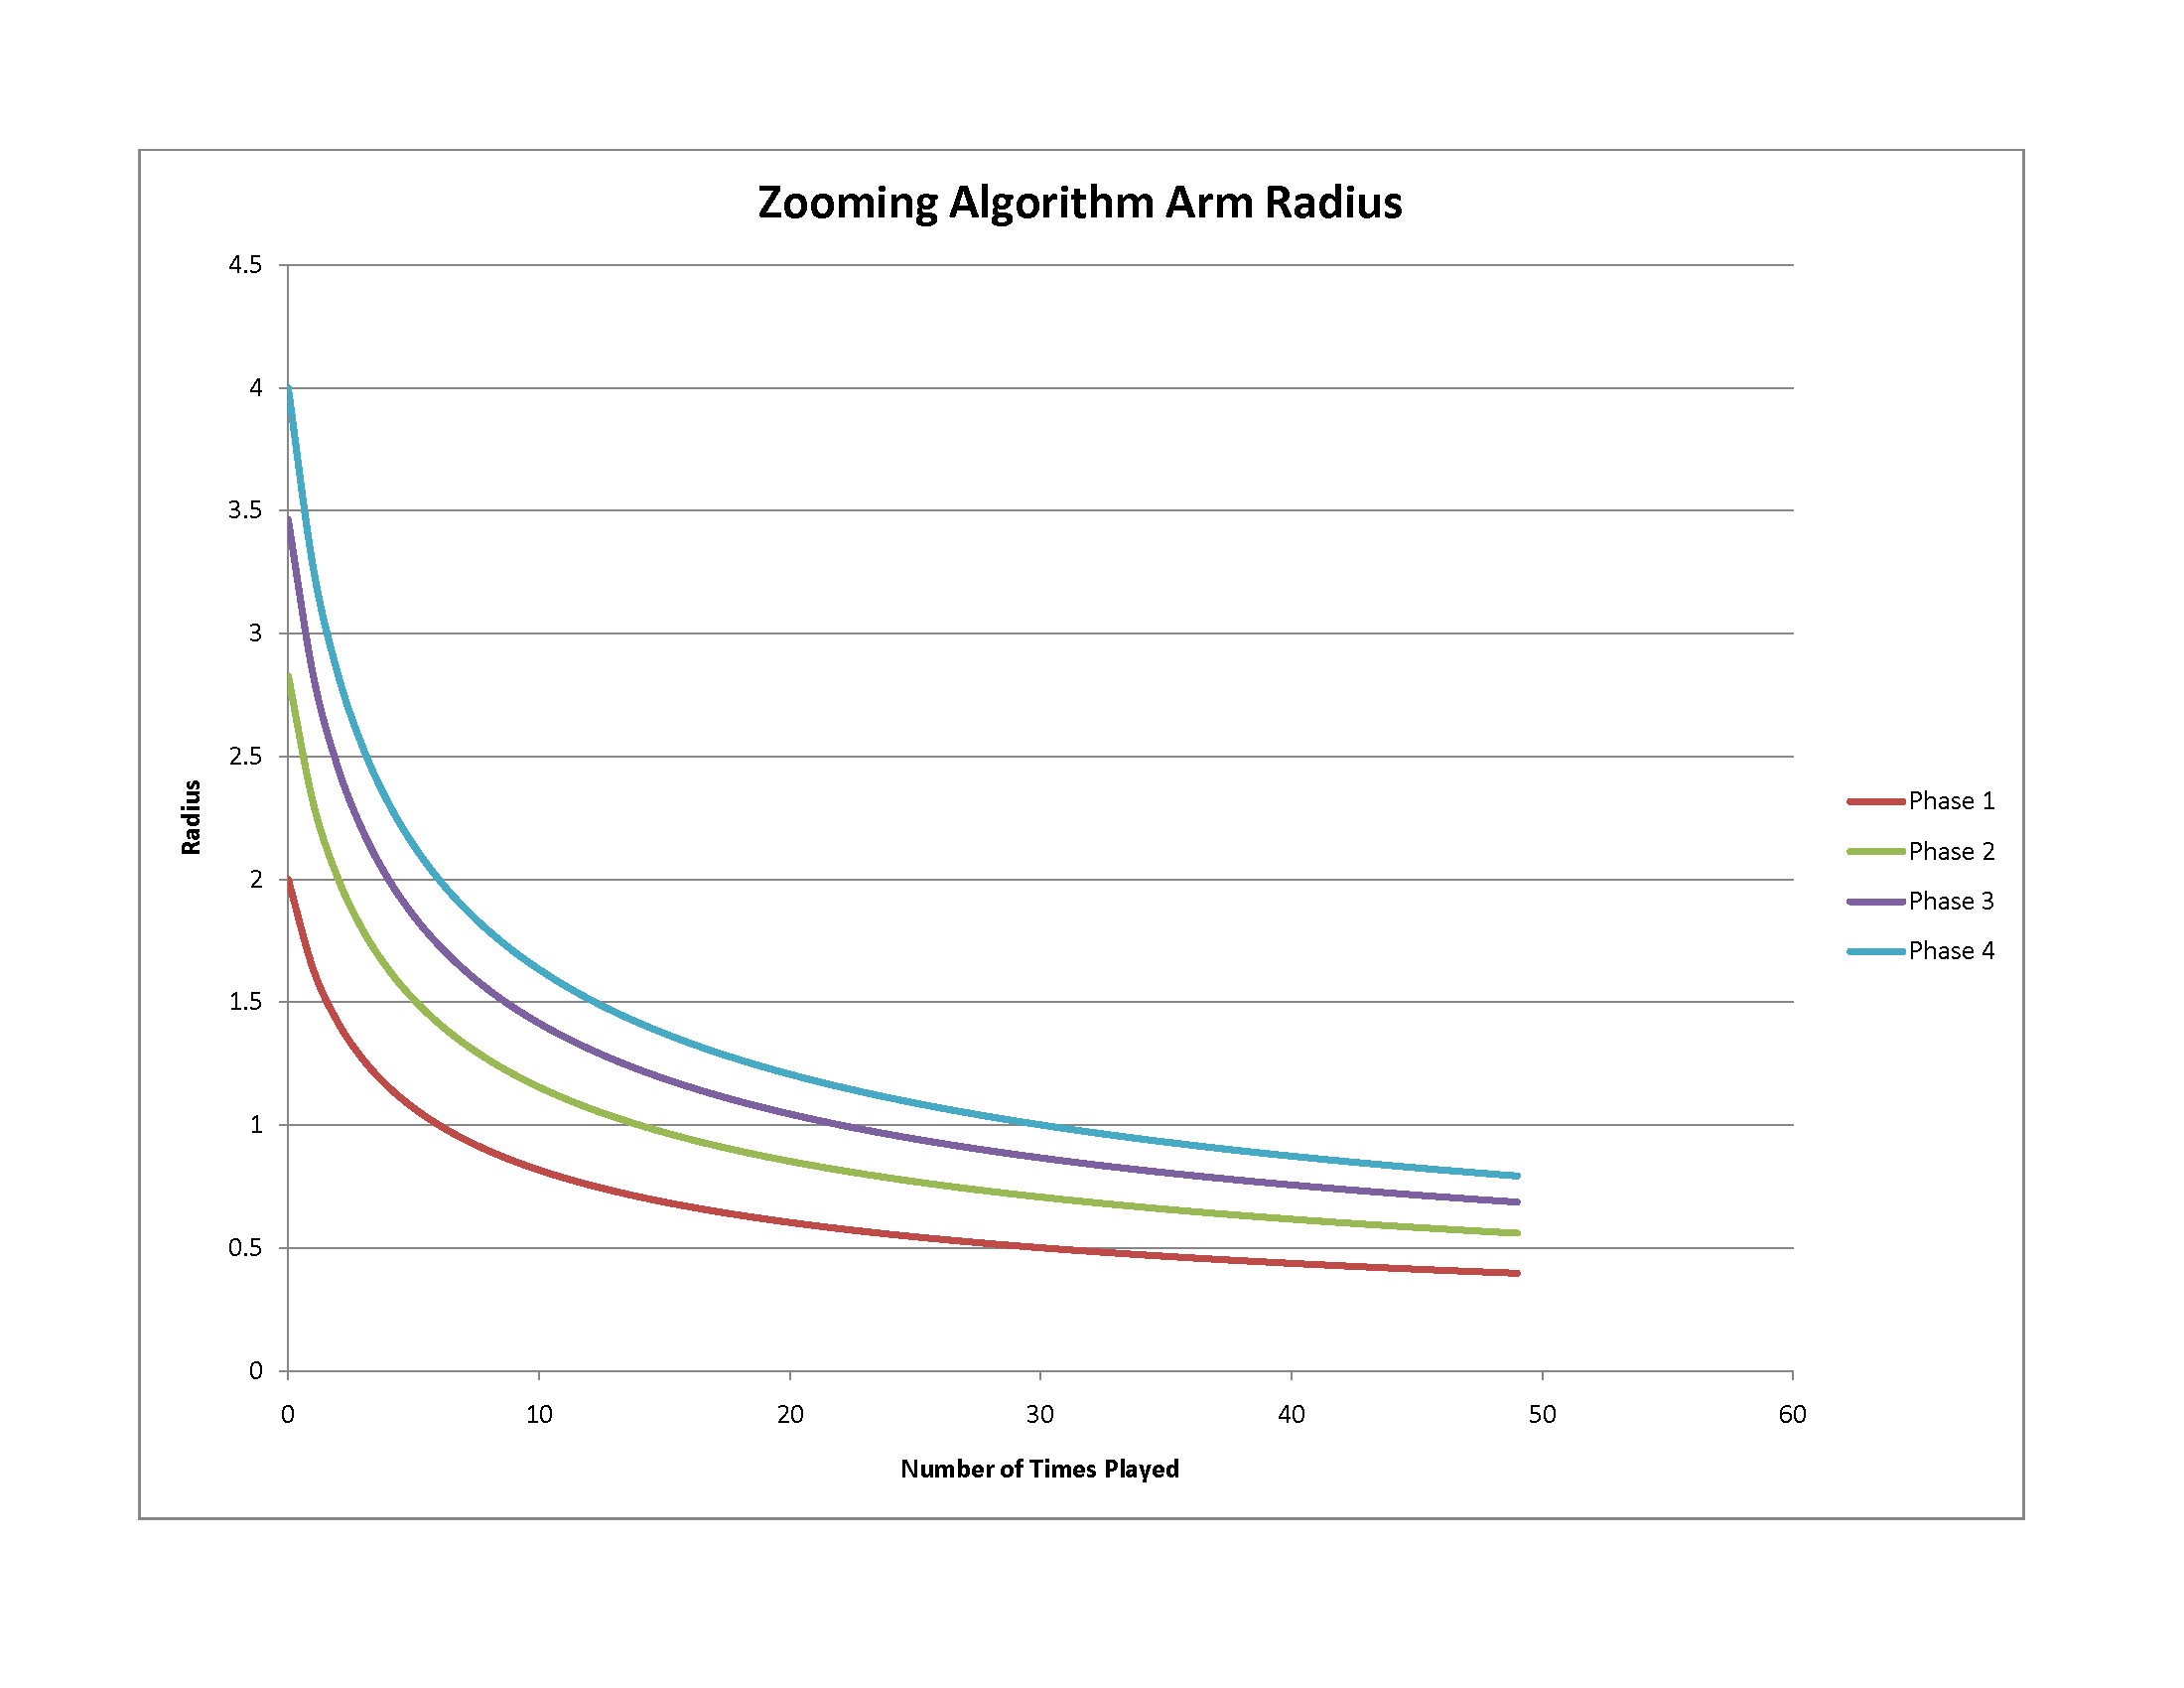
\includegraphics[width=5 in]{figures/ZoomingRadius.png}
     \caption{Arms cover less area the more they are played. The phase
       number only changes the scaling.}
     \label{fig:zoomradius}
  \end{center}
\end{figure}

Inbetween different phases, the Zooming Algorithm does not carry over
information. All that changes is $i_{ph}$. As $i_{ph}$ increases, the
index is effected increasingly more by how many times an arm has been
played. This means that earlier rounds have indices that are more
influenced by the $\mu_t(v)$, and will thus tend to exploit their
earlier finds more, while later rounds will perform more exploration
before zeroing in on the optimal arm. Given specific knowlege about
the problem at hand, this value could be optimized, allowing you to
run the zooming algorithm for a specific phase number.

\begin{figure}[!ht]
  \begin{center}
    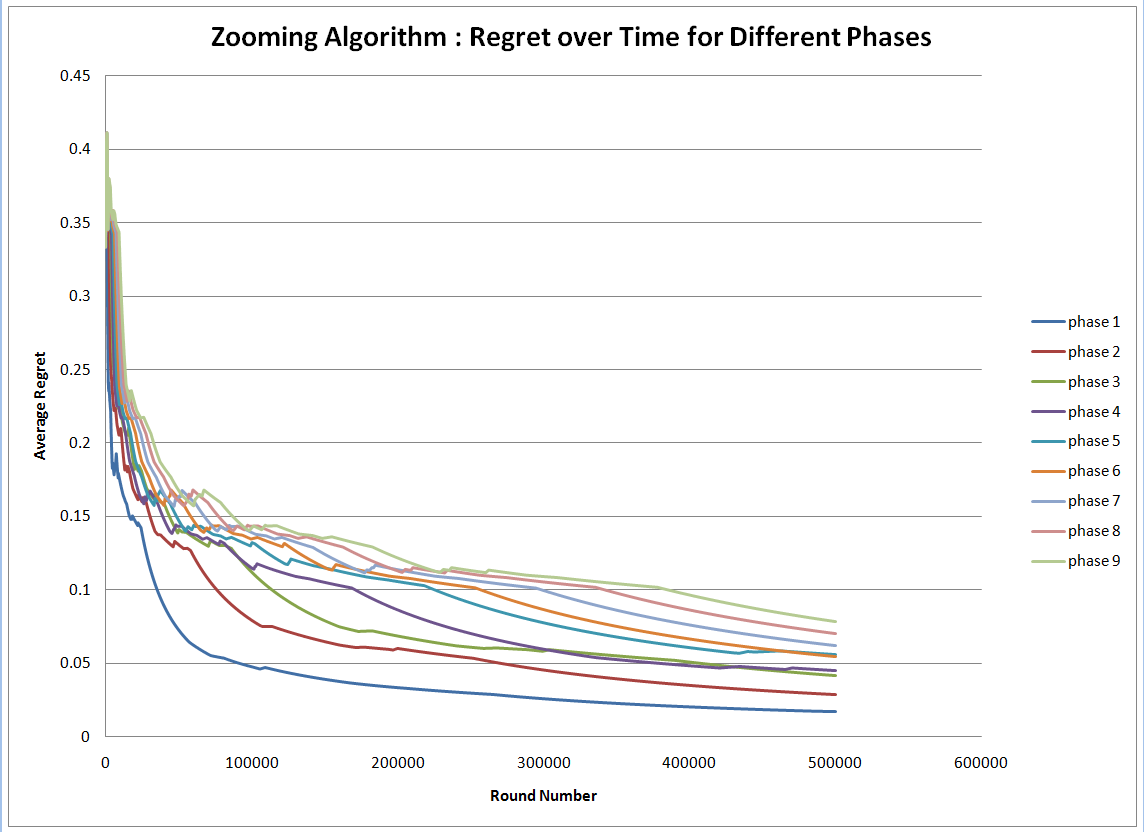
\includegraphics[width=5 in]{figures/Phase_Comparison.png}
     \caption{Here, the Zooming Algorithm was modified to run
       indefinitely on a specific phase number. As you can see, as a
       result of later phases doing more exploration, and having
       larger initial radii for their arms, later phases take longer
       to converge than earlier phases. The algorithm was run on a 2
       dimensional domain from 0 to 1 where reward is maximized at the
       point $(.3,.3)$. Reward was given by
       $\frac{1}{1+\mathrm{d}(v,(.3,.3))}$}
     \label{fig:zoomphase}
  \end{center}
\end{figure}



The runtime of the Zooming Algorithm depends very heavily on how the
covering oracle chosen behaves. This can be problematic, since the problem
is np-complete for the problem of hypercube coverings  \cite{Hoffmann05acovering} . In high dimensions,
the oracle can become quite expensive.

%%%%%%%%%%%%%%%%%%%%%%%%%%%%%%%%%%%%%%%%%%%%%%%%%%%%%%%%%%%%%%%%%%%%%%%%%%%%%
\subsection{Discretization Algorithms}
To test the $\mathcal{X}$-armed and Zooming algorithms, we have
implemented the $\epsilon$-greedy, UCB1 \cite{auer2002finite}, and
Exp3 \cite{auer1995gambling} finite-armed algorithms for the case
where whatever domain our bandit problem is over is discretized into
some finite number $K$ points.  In common to each algorithm is the
fact that the points are chosen randomly and uniformly from the
domain.  The intuition behind this choice is that, otherwise, it would
be relatively easy to construct a reward function that any
discretization would do terribly for, simply by ensuring that the
peaks of the reward function did not occur where the algorithm picked
a point.  For example, if arms were chosen in regular intervals from
the interval [0,1], i.e. at the points $\frac{i}{K+1}$, with $1 \leq i
\leq K$, then a reward function with a sharp peak at 0 would be
guaranteed to make any discretization algorithm perform poorly.
Choosing the arms at random at least guarantees that there is a chance
of doing well.  A brief description of the particulars of each
algorithm is now given.

\subsubsection{$\epsilon$-Greedy}
In round $t$, if $1 \leq t \leq K$ then play arm $t$.  Otherwise, play
randomly with probability $\epsilon$ and the arm with the best running
average otherwise.  We have implemented this algorithm using $\epsilon
= \frac{K}{t}$.

\subsubsection{UCB1}
In round $t$, if $1 \leq i \leq K$ then play arm $i$.  Otherwise, play
the arm that maximizes the quantity
\[
	\bar{r_i} + \sigma \sqrt{\frac{2 \log(t)}{p_i}}
\]
Where $\bar{r_i}$ is the average reward of arm $i$ so far, $p_i$ is the 
number of times arm $i$ has been played so far, and $\sigma$ is a parameter
that can be chosen to influence how much exploration is done.

\subsubsection{Exp3}
Initialize $w_i(1) = 1$ for all $1 \leq i \leq K$.  In round $t$, play
arm $i$ with probability
\[
	p_i(t) = \frac{\epsilon}{K} + (1 - \epsilon) \frac{w_i(t)}{\sum_j w_j(t)}
\]
With $i$ the arm that was played, update
\[
	w_i(t+1) = w_i(t)\gamma^{\frac{\epsilon r_i(t)}{K p_i(t)}}
\]
where $r_i(t)$ is the reward recieved, and set $w_j(t+1) = w_j(t)$ for all
other arms $j$.  $\gamma$ is a parameter that can be chosen to influence how
much exploration is done.  As in the $\epsilon$-greedy algorithm, we use
$\epsilon = \frac{K}{t}$.
